%!TEX encoding = UTF-8 Unicode
% !TeX spellcheck = en_GB
%%%%%%%%%%%%%%%%%%%%%%%%%%%%%%%%%%%%%%
\chapter{The Standard Model Higgs boson }\label{chap:HiggsSM}
%%%%%%%%%%%%%%%%%%%%%%%%%%%%%%%%%%%%%%
%\epigraph{	It's very nice to be right sometimes... it has certainly been a long wait.}{\textit{Peter Higgs }}

\section{Spontaneous symmetry breaking \label{sec:ssb}}
\par Before talking about symmetry breaking, we need to discuss the concept of symmetry in physics. Symmetry is a crucial part of studying physical systems. It manifests not only as a geometric feature of physical objects but also in the dynamics of physical systems. For example, one can find symmetries in the equations of motion, Lagrangians/Hamiltonians and actions. The magnetisation of materials is a good example of symmetry's role in describing physical behaviour. For instance, {paramagnetic} materials have a positive magnetic susceptibility~$\chi_B$ due to the random arrangement of their electrons' spins.  The paramagnetic material spins arrangement will therefore possess rotational symmetry. The material has no \textit{ preferred direction} in space~\cite{minlos2000introduction}. \textit{Au contraire}, {ferromagnetic} materials with the electrons' spins aligned in a certain direction will not have such symmetry as there will be a preferred direction, see~\autoref{fig:paravsferro}. 
%%%%
\begin{figure}[htpb!]
	\centering  
	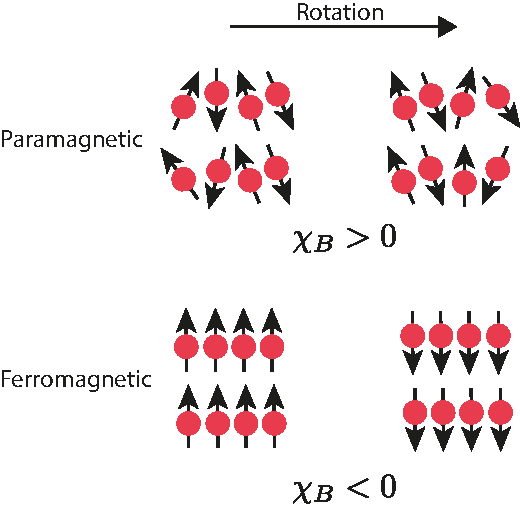
\includegraphics[width=0.36\linewidth]{./figures/ferrvspara}
	\caption{In paramagnetic materials, the spins are randomly distributed such that a rotation performed on the system will keep the spin distribution invariant. However, the symmetry is broken for ferromagnetic materials, where the spins are aligned in a single direction, and the system has a preferred direction.}  \label{fig:paravsferro}
\end{figure}
%%%%
%%%%
\par In particle physics and quantum field theory, symmetry plays an essential role in the taxonomy and dynamics of elementary particles and their bound states, i.e. hadrons, cf.~\cite{osti_4008239,PhysRev.96.191}. There are two types of symmetries considered when studying elementary particles and their quantum fields: external and internal symmetries. The first is the symmetry of the spacetime background. Typically, this is a four-dimensional Poincar\'e symmetry.  Higher spacetime dimensions or non-flat geometries are considered in some models. However, there is no current evidence of higher dimensions or indications of non-flat spacetime from colliders and cosmological observations~\cite{Zyla:2020zbs}. The second class of symmetries is internal symmetries stemming from the quantum nature of these particles/fields. Because their state is described by a {ray} in complex Hilbert/Fock spaces, internal symmetries are simply symmetries of rotations in these spaces that keep the action variation unchanged. Internal symmetries are usually described in terms of simple or product of simple {Lie groups}, e.g. $SU(N)$~\footnote{Gauge theories based on finite groups have been proposed in the literature, but their phenomenological significance is yet to be further investigated~\cite{Freed1993LecturesOT,dijkgraaf1990topological}}. Particles/fields will be arranged as multiplets in some representation of the groups. If the rotations of the states could be parametrised by constants, the symmetry is called {global}. Alternatively, if these transformations are themselves functions of the spacetime,  the symmetry is then called {local} or \textbf{gauged}.
%%%%
\par Gauge symmetries describe rotations in the state of space that depends on spacetime. The generator of the gauge transformations could propagate between two spacetime points. This is the way particle interactions are described in quantum field theory. The generators of these gauge transformations are called gauge bosons, and they mediate the interactions between the particles and hence transform under the adjoint representation of the gauge group. Gauge symmetries are the basis of describing the fundamental interactions of nature,  called gauge theories.
%%%%
\par An example of a gauge theory that is realised in nature is the \textbf{Standard Model}~(SM), which is a gauge theory based on the group~$G_{\SM}:=SU(3)_C \otimes SU(2)_L \otimes U(1)_Y$. The first simple group is for the \textit{strong} interaction described by quantum chromodynamics~(QCD). The product of the two remaining groups~$SU(2)_L \otimes U(1)_Y$ forms the Weinberg-Salam \textit{electroweak}~(EW) model~\cite{salam2,salam1,PhysRevLett.19.1264}, where~$SU(2)_L$ describes the weak interaction which only couples to \emph{left handed} fermions and $U(1)_Y$ is the weak hypercharge~$Y$ gauge group, defined by the formula
\begin{equation}
	Y= 2(Q-T_3).
\end{equation}
Where $Q$ is the electric charge and $T_3$ is the third component of the weak isospin. A description of the matter content of the SM and their multiplicities with respect to~$G_{\SM}$ is shown in~\autoref{tab:thesm}
%%%%
\begin{table}[htpb!]
	\centering
	\begin{tabular}{ccl}
		\topline
		\rowcolor{tableheadcolor} Particle/Field& $G_\SM$ multiplicity& \multicolumn{1}{c}{mass [\si{\GeV}]}  \\
		\midtopline
		\topmidheader{3}{\textbf{Quarks}} 
		$Q = {u_L \choose d_L},{c_L \choose s_L},{t_L \choose b_L}$ & $(\irrep{3},\irrep{2})_{1\over 6}$ & $m_u=2.16\cdot10^{-3}$, $m_d=2.67\cdot10^{-3}$\\
		$U= u_R, c_R, t_R$ & $(\irrep{3},\irrep{1})_{2\over3}$&$m_c=0.93\cdot10^{-2}$, $m_s=1.27$\\
		$D= d_R, s_R, b_R$ & $(\irrep{3},\irrep{1})_{-{1\over3}}$&$m_t=172.4$, $m_b=4.18$\\
		\midrule
		\topmidheader{3}{\textbf{Leptons}} 
		$L = {\nu_{e,L} \choose e_L},{\nu_{\mu,L} \choose \mu_L},{\nu_{\tau,L} \choose \tau_L}$ & $(\irrep{1},\irrep{2})_{-{1\over2}}$ & $m_e=0.511\cdot10^{-3}$, $m_\mu=1.05\cdot10^{-2}$\\
		$E= e_R, \mu_R, \tau_R$ & $(\irrep{1},\irrep{1})_{-1}$&$m_\tau=1.77$,$m_\nu=$??\\
		\midrule
		\topmidheader{3}{\textbf{Gauge bosons}} 
		$g/G^A_\mu,\,\,\, A=1\dots 8$ &$(\irrep{8},\irrep{1})_{0}$& \multicolumn{1}{c}{$ 0.0$}\\
		$\gamma/A_\mu$ &$(\irrep{1},\irrep{1})_{0}$& \multicolumn{1}{c}{$ 0.0$}\\
		$W^\pm_\mu$ &$(\irrep{1},\irrep{3})_{0}$& \multicolumn{1}{c}{$ 80.379$}\\
		$Z_\mu$ &$(\irrep{1},\irrep{3})_{0}$& \multicolumn{1}{c}{$ 91.1876$}\\
		\midrule
		\topmidheader{3}{\textbf{The Higgs boson}} 
		$h$ &$(\irrep{1},\irrep{2})_{1\over 2}$& \multicolumn{1}{c}{$ 125.10$}\\
		\bottomline
	\end{tabular}   
	\caption{The SM constituents, their multiplicities with respect to the SM gauge group ~$G_{\SM}:=SU(3)_C \otimes SU(2)_L \otimes U(1)_Y$ and masses. The mass of the neutrinos $\nu$ is zero according to the SM prediction, but observations suggest that they are massive, and only the difference between the three masses is known~\cite{Capozzi:2016rtj}. The values of the masses are taken from the Particle Data Group~(PDG)~\cite{Zyla:2020zbs}, and used throughout this thesis.}\label{tab:thesm}
\end{table}

%%%%
%%%%
\par The SM has been very successful at describing particle interactions even when challenged by numerous precision tests at LEP and SLD~\cite{ALEPH:2005ab,SLD:2000jop,Group:2012gb,ALEPH:2013dgf}. Later at D\O~\cite{2011baz} and the LHC~\cite{CMS:2014mgj,ATLAS:2017rzl} Nevertheless, it fails to describe the ground state if only the fermion and gauge sectors are considered. This shortcoming is that the $W^\pm$ and $Z$ bosons are massive. This violates the EW gauge symmetry. This can be easily seen by looking at the mass term of a spin one field $B^A_\mu$
\begin{equation}
	\mathcal{L} = m_B B^{A,\mu}B^A_\mu,
\end{equation}
and performing an $SU(N)$ gauge transformation 
\begin{equation}
	B^A_\mu \to B^A_\mu+\partial_\mu \Lambda ^A+g \,\varepsilon^A_{BC} B^B_\mu \Lambda^C.
\end{equation}
We see that the mass term does not preserve gauge symmetry.
Secondly, because the SM is a chiral theory, only left-handed fermions are doublets under~$SU(2)_L$. Thus, the Dirac mass term
\begin{equation}
	\mathcal{L}_{\mathrm{D}} = m_D \bar \psi_L \psi_R+ \hc,
\end{equation}          
cannot be a singlet under~$SU(2)_L$, this again violates the EW symmetry. Despite quark and lepton masses being forbidden by the EW symmetry, we have already measured them, and since they also carry charges, this mass has to come from a Dirac mass term. 
\par For the EW model to be consistent in the ground state like it is in the interaction states. A mechanism for spontaneous symmetry breaking~(SSB) needed to be introduced. 
%%%%%%
\subsection{Nambu-Goldstone theorem}
%%%%%%%
Coming back to the example of the paramagnetic-ferromagnetic materials, when a ferromagnetic metal is heated above a certain temperature, known as the~{Curie Temperature}~$T_C$, it will undergo a phase transition and become paramagnetic. In the mean-field theory approximation, the magnetic susceptibility is related to the temperature of the metal via the relation
\begin{equation}
	\chi_B \sim (T-T_C)^{-\gamma},
\end{equation}  
where $\gamma$ is called a critical exponent. We see that if the metal temperature is $T>T_C$; the metal is in an~\textit{disordered phase} and when it is $T<T_C$, the metals becomes in the~\textit{ordered phase}, i.e. $\chi_B$ is the {order parameter} of this system. At the Curie temperature, the system will be at the~\textit{critical point}, and the susceptibility is divergent. The exponent~$\gamma$ cannot be used to describe the system at the critical point. \\ There is a ``pictorial'' description of the metal at the critical point, which helps understand the Nambu-Goldstone theorem. Starting at $T>T_C$, the metal would be in a paramagnetic phase, where the spins are randomly arranged. As the temperature becomes lower and lower, thermal fluctuations start to lessen. In some regions of the metal, the spins will start to get aligned. With continued cooling, nearing $T_C$, these turned spins will affect their neighbours by flipping their direction. At the critical point $T=T_C$, the system behaves peculiarly when one would see regions of spins in ``up'' and others in ``down'' directions. The system will resemble a fractal of these regions, becoming scale-invariant. Additionally, waves of oscillating local magnetisation will propagate. These waves, or spinless quasiparticles (called {Magnons}), are Goldstone bosons emerging from SSB that manifests at $T<T_C$ as the spins will be arranged in a certain single direction and the metal becomes ferromagnetic.
\begin{tcolorbox}[title=The Nambu-Goldstone theorem,
	title filled=false,
	colback=Mahogany!5!white,
	colframe=Mahogany]
	When a continuous symmetry has a conserved current but broken in the ground state~(vacuum) is called to be spontaneously broken. A scalar boson is associated with each broken generator of this spontaneously broken symmetry. The modes of these bosons are fluctuations of the order parameter.
\end{tcolorbox}
This theorem first emerged from condensed matter physics, particularly superconductors~\cite{PhysRev.117.648,goldstone}. However, it soon got applied to relativistic quantum field theories~\cite{PhysRev.127.965}.
%%%%%%
\section{The Braut-Englert-Higgs mechanism \label{Higgsmech}}
%%%%%%
To solve the aforementioned shortcomings of the Weinberg-Salam model, the Nambu-Goldstone theorem has been first proposed by P.~W.~Anderson~\cite{PhysRev.130.439}. However, the way that Anderson formulated his theory was unfamiliar to particle physicists and used a non-relativistic picture to illustrate how photons could gain mass in an electron plasma with a plasma frequency $\omega_{p}$ 
\begin{equation}
	m_\gamma^{\mathrm{plasma}} =\frac{\hbar \omega_p}{c^2}.
\end{equation}
Later on, a theory that explains the mass generation of the EW gauge bosons was published in an almost simultaneous manner by R.~Braut~ and F.~Englert~\cite{PhysRevLett.13.321}, P.~Higgs~\cite{PhysRevLett.13.508,HIGGS1964132} and G.~Guralnik, C.~R.~Hagen, and T.~Kibble~\cite{PhysRevLett.13.585,Guralnik:2009jd}\footnote{All of these authors have contributed to the theory of SM ~(SSB). By calling it the ``Braut-Englert-Higgs'' mechanism or the ``Higgs'' boson. I, by no means, have intended to ignore the role played by the rest; rather, I wanted to stick to the most widely-used terminology in the field.}.
The Higgs mechanism starts by considering the SSB of the electroweak sector of the SM via the pattern
\begin{equation}
	SU(2)_L \otimes U(1)_Y \longrightarrow U(1)_{Q} .
\end{equation}
\begin{figure}[t!]
	\begin{center}
		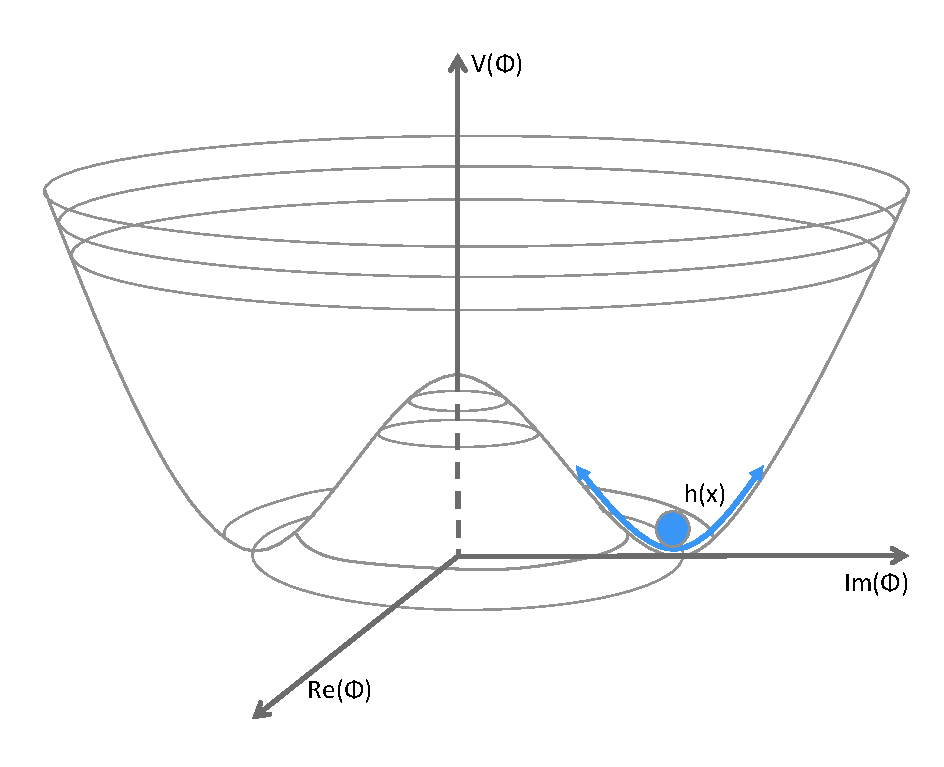
\includegraphics[width=8cm]{figures/HiggsPotential}
		\caption{The characteristic shape of the Higgs potential showing a non-zero vacuum. The physical Higgs boson is an oscillation within the energy well illustrated in the diagram with blue arrows., this illustration is taken from~\cite{Erler:2019hds}. \label{fig:higgs_hat} }
	\end{center}
\end{figure}
This is  achieved by the vacuum expectation value~(vev) of a complex scalar field $\phi\sim (\irrep{1},\irrep{2},+1/2)$, with the Lagrangian 
\begin{equation}
	\mathcal{L} = D_\mu \phi^* D^\mu \phi -V[\phi],\;\;\;\;\;\; V[\phi]:= \mu^2  \phi^* \phi +\lambda (\phi^* \phi)^2,
	\label{higgspot}
\end{equation}
with $V[\phi]$ denoting the Higgs potential, illustrated in~\autoref{fig:higgs_hat}, and generating a non-vanishing vacuum for $ \mu^2 <0$ . The field $\phi$ is given explicitly by 
\begin{equation}
	\phi = \begin{pmatrix}
		\phi^1 + i \phi^2\\  \frac{1}{\sqrt{2}}(h+v)-i \phi^3.
	\end{pmatrix}
\end{equation}
The covariant derivative 
\begin{equation}
	D_\mu= \partial_\mu -ig_2\frac{\sigma_a}{2}W^a_\mu-ig_1\frac{1}{2} B_\mu,   
\end{equation}
dictates the coupling between the Higgs field and the EW gauge bosons and~$g_3$, $g_2$ and $g_1$ are, respectively, the coupling constants of 
${ SU(3)_C}$,  ${ SU(2)_L}$ and  ${ U(1)_Y}$.  
The minimum of the scalar potential is obtained by
\begin{equation}
	\frac{\partial V}{\partial \phi} \mid_{\phi\to v} = 0,
\end{equation}
which for a tachyonic mass~$\mu^2 < 0$ will have a real non-vanishing values~$v$ corresponding to the vev of this field~$\langle \phi \rangle ={0\choose \frac{v}{\sqrt{2}}}$.\\
According to the Nambu-Goldstone theorem, the three broken generators of~$SU(2)_L \otimes U(1)_Y$ will become massive, and they are the $W^\pm$ and $Z$ bosons, while the photon will remain massless. We will have three massless Goldstone bosons $ G^\pm=\frac{1}{2} (\phi^1\pm i\phi^2) $ and $G^0=\phi^3$ that are ``eaten'' by those as mentioned earlier massive $W^\pm$ and $Z$ bosons, where these Goldstone bosons become the longitudinal polarisations of  $W^\pm$ and $Z$. To see this more concretely, we start by looking at the terms of the EW Lagrangian, where the field $\phi$ couples to the gauge bosons in the unbroken phase
\begin{equation}
	D_\mu \phi^* D^\mu \phi = \frac{1}{2} |\partial_\mu \phi|^2 + \frac{1}{8}g_2^2|\phi|^2|W_\mu^1+iW_\mu^2|^2
	+ \frac{1}{8}|\phi|^2 |g_2 W_\mu^3- g_1 B_\mu|^2.
	\label{ewhiggs_ub}
\end{equation}
After SSB, we have the gauge bosons in the mass basis~
\begin{align}
	W_\mu^\pm &= \frac{1}{\sqrt{2}} (W^1_\mu\pm iW^2_\mu), \nonumber \\
	Z_\mu &= \frac{1}{\sqrt{g_1^2+g_2^2}} \left(g_2 W^3_\mu-g_1B_\mu\right), \\
	A_\mu &= \frac{1}{\sqrt{g_1^2+g_2^2}} \left(g_2 W^3_\mu+g_1B_\mu\right). \nonumber
\end{align}
From this, the electric change is identified as the coupling constant to the photon~$A_\mu$ 
\begin{equation}
	e=\frac{g_1}{\sqrt{g_1^2+g_2^2}}.
\end{equation}
It is useful to define the~{Weinberg angle}~$\theta_W$, an important EW parameter relating the electric charge to the weak coupling~$g_2$ 
\begin{equation}
	\sin \theta_W = \frac{e}{g_2} \approx 0.231214,
\end{equation}
typically the $\sin$ and $\cos$ of the Weinberg angle are denoted by $s_W$ and $c_W$, respectively. \\ We use the unitary gauge, to absorb the Goldstone bosons into the $W^\pm$ and $Z$ longitudinal polarisations. In this gauge the Higgs doublet can be written as
\begin{equation}
	\phi \to \begin{pmatrix}
		0\\  \frac{1}{\sqrt{2}}(h+v).
	\end{pmatrix}, \,\,\,\,\,\,\,\, v= 246\, \mathrm{GeV}.
	\label{unitaryhiggs}
\end{equation}
With these substitutions, one can read off the masses of the gauge bosons from their bilinear terms in~\eqref{ewhiggs_ub}
\begin{align}
	m_W =& \frac{vg_2}{2} & m_Z&=\frac{v}{2}\sqrt{g_1^2+g_2^2} & m_A &= 0.
\end{align}
Since $\phi$ is a complex scalar doublet, it has four components,  three of which correspond to the Goldstone bosons; one remains as a physical field~$h(x)$, which is identified as the ``Higgs boson'' discovered in the Summer of 2012~\cite{CMS:2012qbp,ATLAS:2012yve}. The couplings between  the Higgs boson and the electroweak bosons are related to their mass via the vev 
\begin{align}
	g_{hVV} =& \frac{2 m_V^2}{v}, & g_{hhVV}=& \frac{2 m_V^2}{v^2}.
\end{align}
By substituting~\eqref{unitaryhiggs}, into the Higgs potential~\eqref{higgspot} one can also write the mass of the physical Higgs boson in terms of the vev
\begin{align}
	m_h =\sqrt{2 \lambda} v .
\end{align}
The  Higgs boson mass is related to the $\mu$ parameter via the relation
\begin{align}
	m_h ^2 =-2 \mu^2,
\end{align}
One can see that the mass term after SSB changes its sign, characterising the order parameter for this system,  analogous to the magnetic susceptibility for the magnetisation of materials example. 
One could also identify the self-couplings of~$h$, the trilinear and quartic couplings 
\begin{align}
	g_{hhh}&=3\lambda v =3\frac{m_h^2}{v}, & g_{hhhh}&= 3 \lambda = 3\frac{m_h^2}{v^2}.
\end{align}
%%%
\section{Yukawa interaction \label{smyukawa}}
It is possible to also use the Higgs vev to give fermions their masses by introducing  Yukawa-interaction terms, first introduced by S. Weinberg~\cite{PhysRevLett.19.1264}
\begin{equation}
	\mathcal{L}_{\mathrm{Yuk}}= -y_{e} \, \bar{L} \, \phi \, E 
	- y_{d} \, \bar{Q} \, \phi \, D
	- y_u \, \bar{Q} \, \tilde{\phi} \, U   \ + \hc,
	\label{lag-yuk}
\end{equation}
with $ \tilde{\phi}= i\sigma_2 \phi$ and $ y_e, y_d, y_u$ are $3\times 3$ matrices. These matrices are free parameters in the SM. As the Higgs boson acquires a vev, the fermions will acquire a mass $m_f= vy^\prime_f$ and the Higgs boson coupling to the fermions is given by
\begin{equation}
	g_{h\bar{f}f} = \frac{m_f}{v},
\end{equation}
and the Yukawa matrices will be fixed in the mass basis ~$y^\prime_f$ by measurements of the fermion masses.\\  Leptonic Yukawa matrix is diagonal, with a degeneracy between the flavour and mass basis, this manifests as lepton family number conservation. That is, the lepton family operator commutes with the Hamiltonian. However, for the quarks, the situation is more complicated. One can rotate these matrices to the mass basis via a bi-unitary transformation via the unitary matrices~$ \mathcal{V}_q, \mathcal{U}_q$ for $ q= u,d$
\begin{equation}
	y_{q} \longrightarrow y^\prime_q= \mathcal{V}^\dagger_{q} \,y_q\, \mathcal{U}_{q} = \text{diag}\left(m_{q_1}, m_{q_2},m_{q_3}\right).
\end{equation}
The is no degeneracy here as the Hamiltonian does not commute with the quark flavour operator. The transformation matrices for the up and down-type quarks are not the same.  The charged EW quark currents contain flavour mixing described by the Kabibbo-Kobayashi-Maskawa~(CKM) matrix~\cite{PhysRevLett.10.531,10.1143/PTP.49.652}. 
\autoref{fig:SMcouplings} shows all the SM couplings' strengths, with the thickness of the chord is proportional to the strength of the coupling; the Higgs couplings are highlighted in orange. 
%%%%
\begin{figure}[htpb!]
	\centering
	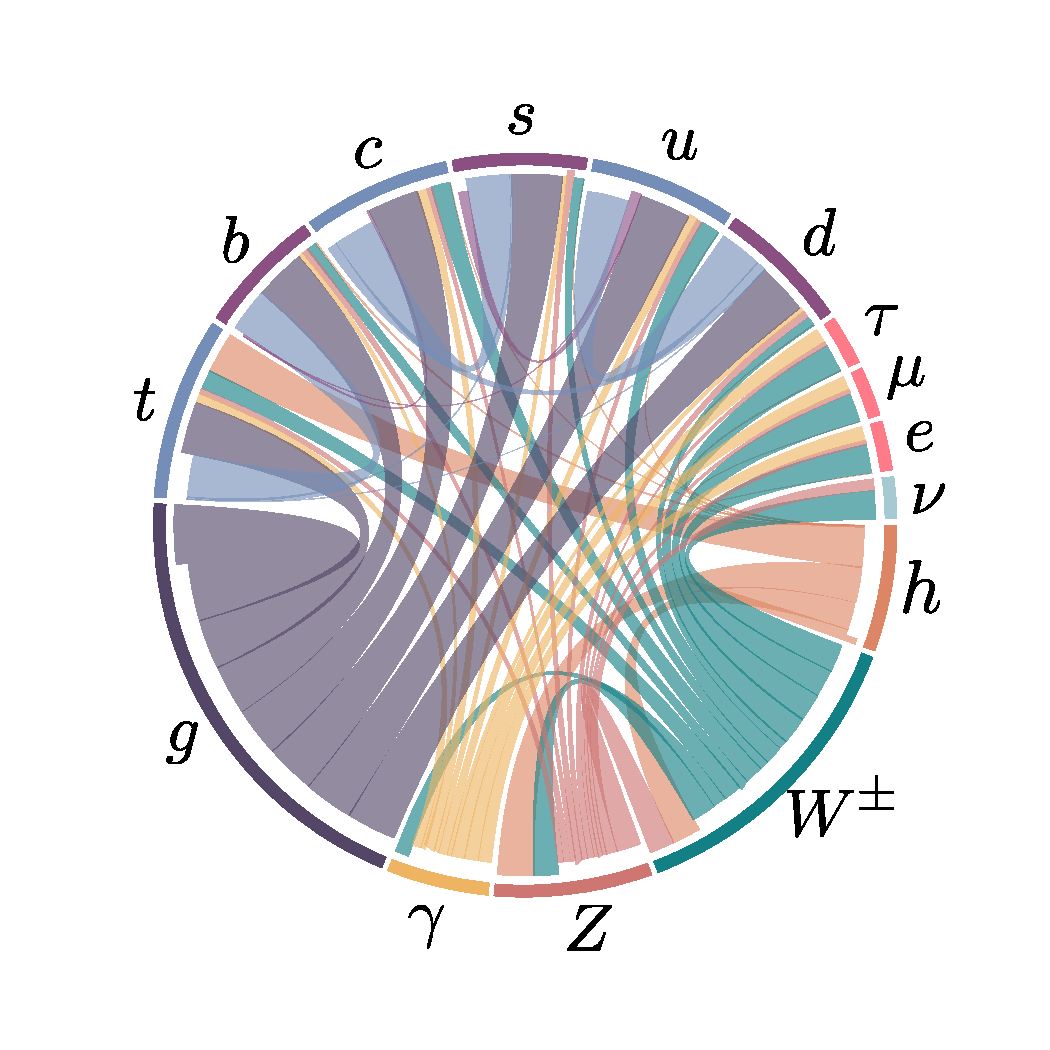
\includegraphics[width=\linewidth]{./figures/SM}
	\caption{A chord diagram showing the SM couplings, with the coupling strength illustrated by the chord thickness. Higgs couplings are coloured in orange.} \label{fig:SMcouplings}
\end{figure}
%%%%
In this figure, one cannot easily see Higgs coupling to the fermions, except for its couplings to the third generation. Strictly speaking, if we further examined the Yukawa coupling using a logarithmic scale and focused on the quark sector as ~\autoref{fig:SMYuk} illustrates. These Yukawa couplings span about six orders of magnitude with a marked hierarchy. These couplings are, in fact, free parameters in the SM and only determined by the experimental measurements of the quark masses. This hierarchy of quark masses, therefore, cannot be explained by the SM Braut-Englert-Higgs mechanism and is sometimes known as \text{the ``old'' flavour puzzle}.  \\ In later chapters, we will examine the experimental effort to measure these couplings better and how Higgs pair production can be used to probe them in~\autoref{chap:lightyuk}. Even the potential of using techniques from \emph{interpretable machine learning} to further improve Higgs pair sensitivity to probing light quarks Yukawa couplings.
\begin{figure}[htpb!]
	\centering
	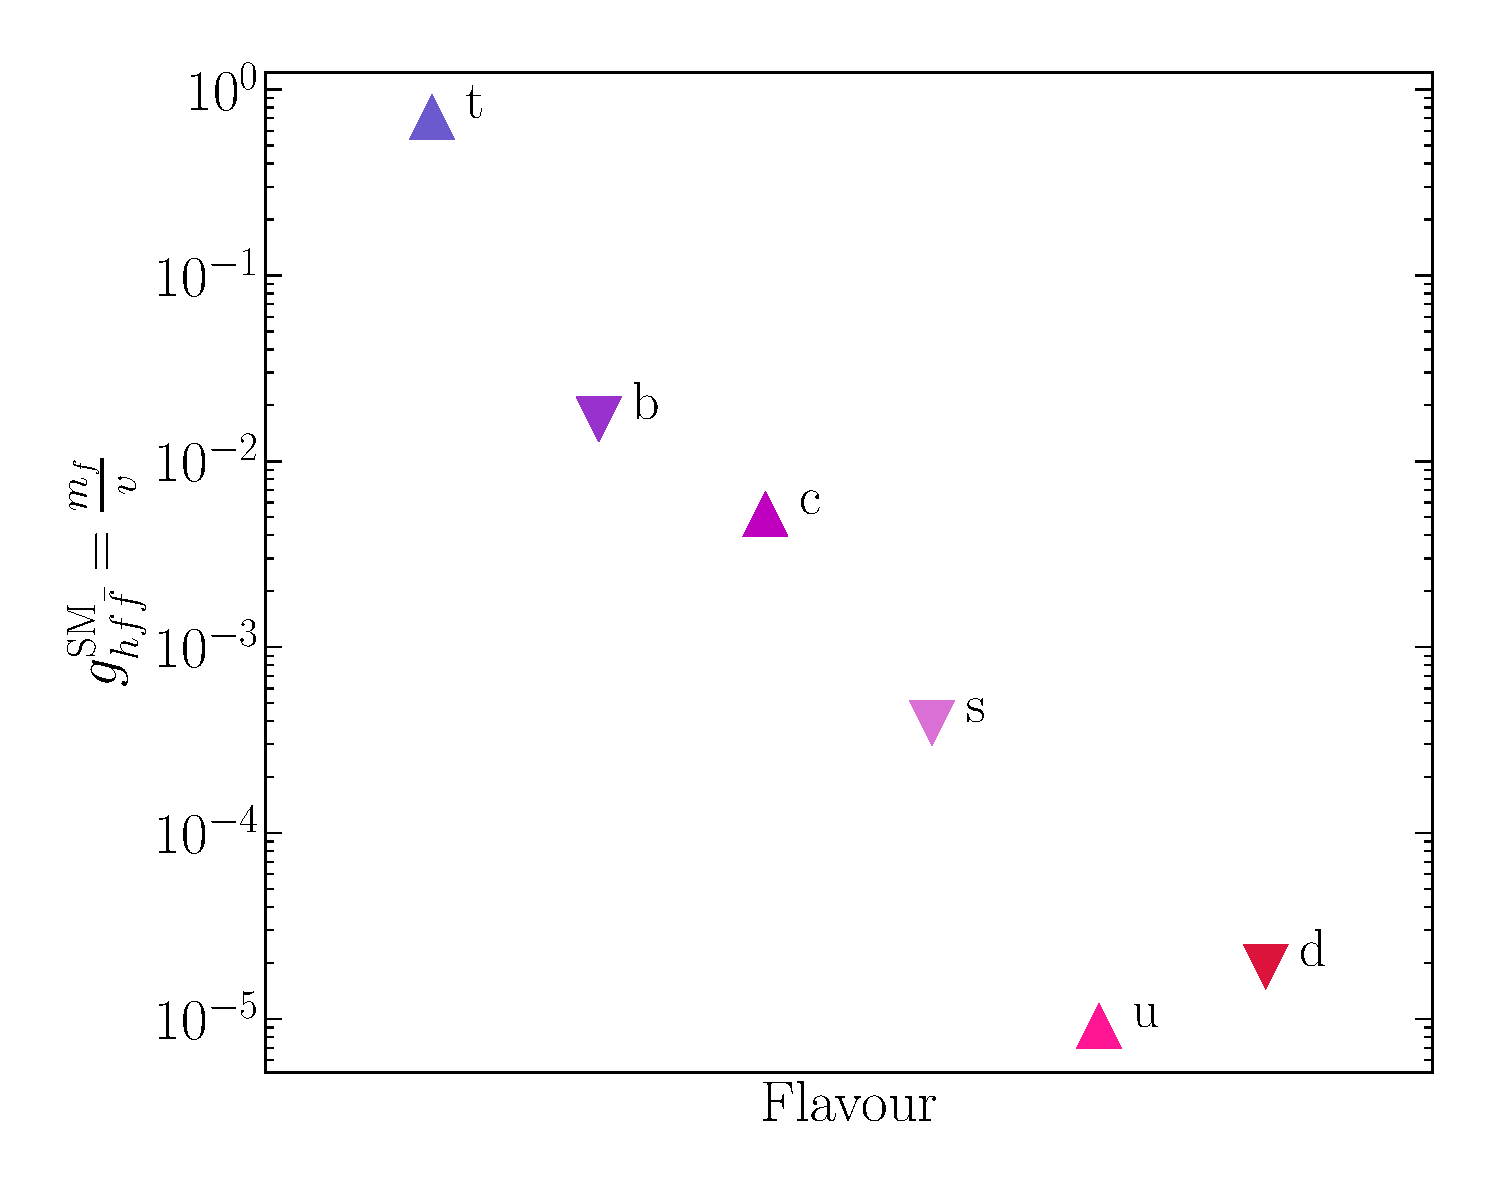
\includegraphics[width=0.5\linewidth]{./figures/yukawa}
	\caption{The SM Yukawa couplings are proportional to the quark masses because the Higgs Yukawa couplings span about six orders of magnitude, as seen in the case of quarks here. The SM cannot explain this large hierarchy. } 
	\label{fig:SMYuk}
\end{figure}
\section{The Higgs and EW precision observables}
One of the most valuable sources for studying new physics (NP) above the EW scale is provided by indirect tests of the SM via the so-called EW precision observables (EWPO). These include, in particular, the very precise measurements at the $Z$ pole performed at the Large Electron-Positron collider (LEP) and the Stanford Linear Collider (SLC). In corroboration with the Higgs boson discovery and the experimental information collected at LHC and Tevatron, they provide strong constraints on theories beyond the SM (BSM) that lead to significant deformations of the standard EW sector~\cite{Falkowski:2013dza,Ciuchini:2013pca,Falkowski:2014tna,deBlas:2015aea,deBlas:2016ojx,deBlas:2017wmn,Haller:2018nnx,Ellis:2018gqa,Erler:2019hds,Dawson:2020oco}.
\par Higgs physics is deeply intertwined with the EW sector as many of the Higgs parameters are linked to EWPO. For instance, the Higgs vev is determined from Fermi's constant~$v =(\sqrt{2}G_F)^{-1/2}$, which is in tern fixed by the muon lifetime~$ \tau_\mu$ measurements~\cite{PhysRev.101.866,PhysRev.113.1652,Mohammad:1976qd,PhysRevLett.82.488}. This can be seen when we examine the theoretical prediction for $ \tau_\mu$ 
\begin{equation}
	\tau_\mu^{-1} = \frac{G_F^2 m_\mu^5}{192\pi^3}\left(1-\frac{8 m_e^2}{m_\mu}\right) \left[1-1.810\frac{\alpha}{\pi}+(6.701\pm0.002)\left(\frac{\alpha}{\pi}\right)^2\right],
\end{equation}
then comparing this formula with the experimental measurements of~$ \tau_\mu$. This confrontation leads to a very precise measurement on $G_F$~\cite{Zyla:2020zbs}
\begin{equation}
	G_F=1.1663787(6) \cdot 10^{-5} \si{\per\GeV\squared},
\end{equation}
given the value of the fine structure constant~$\alpha^{-1} =137.03599976 (50)$. 
\par Another important EWPO is the ratio between the $W$ and $Z$ masses
\begin{equation}
	\rho = \frac{m_W^2}{c_W^2m_Z^2}.
\end{equation}
At leading order~(LO), this parameter is equal to unity in the SM. The $\rho$ parameter depends on the representation of the scalar sector of the EW model. If one supplements the SM EW sector with $\phi_i$ scalars having $T_i$ weak isospin and $T_{3,i}$ being its third component; each of these scalars acquires a vev $v_i$. Then the $\rho$ parameters can be estimated based on these properties via the relation~\cite{ROSS1975135,Djouadi:2005gi}
\begin{equation}
	\rho =\frac{\sum_i [T_{i}(T_{i}+1)-T_{3,i}^2]v_i^2}{2\sum_i T_{3,i}^2v_i^2}.
	\label{rhohiggs}
\end{equation}
From~\eqref{rhohiggs} one can see that a real triplet scalar, for instance, would not fit the experimental EW measurement of $\rho$. Rather, a complex doublet is the simplest scalar possible for the EW symmetry breaking.\\ Radiative corrections to the EW gauge bosons mass from vacuum polarisation diagrams could potentially cause $\rho$ to deviate significantly from unity.  This is not the case, as the experimentally measured value of~$\rho$~\cite{Zyla:2020zbs} of:
\begin{equation}
	\rho_{\text{exp}} = 1.00038 \pm 0.00020.
	\label{eq:rhoexp}
\end{equation}
Additionally, it is possible to think of an extended Higgs sector, where there are multiple scalars with different $SU(2)_L$ multiplicities. Or a composite Higgs sector, in which the Higgs boson is a pseudo-Nambu-Goldstone boson, cf.~\cite{Dugan1985AnatomyOA,Hill:2002ap}. How can such models be built assuring the $\rho$ parameter is protected from change? The answer to this question lies in a symmetry of the Higgs Lagrangian known as custodial symmetry. 
\subsection{Custodial symmetry}
After SSB, a residual global symmetry known as the custodial symmetry protects the $\rho$ parameter from obtaining large radiative corrections at higher orders in perturbation theory.  This symmetry must be kept in extended or composite Higgs models, in order to ``survive'' the current experimental constraints. This symmetry can be seen by rewriting the Higgs potential as
\begin{equation}
	V = \frac{\lambda}{4} \left( \phi_1^2+\phi^2_2+\phi_3^2+\phi^2_4 -2 \mu^2\right)^2.
\end{equation}
This potential is invariant under $SO(4)\simeq SU(2)_L \otimes SU(2)_R$ rotations. However, when the Higgs field acquires a non-vanishing vev,  $ \phi_4 \to h+v$, the potential becomes
\begin{equation}
	V = \frac{\lambda}{4} \left( \phi_1^2+\phi^2_2+\phi_3^2+ h^2+2vh+v^2 -2 \mu^2\right)^2,
\end{equation}
which is only invariant under  $SO(3)\simeq SU(2)_V$ transformations, i.e. the diagonal part of the original group. This global SSB pattern comes alongside the EW-SSB of the gauge group $SU(2)_L \otimes U(1)_Y$ as global $SU(2)_L$ is itself the gauged $SU(2)_L$  group. Additionally, the $T_3$ component of the ~$SU(2)_R$ global group is the gauged $U(1)_Y$, and the~$T^3$ component of the custodial group~$SU(2)_V$ is gauged as well and identified to be the electric charge operator, i.e. the generator of $U(1)_Q$. 
\begin{equation}
	\underbrace{SU(2)_R}_{{\color{myblue} \supset\, U(1)_Y}} \otimes \overbrace{SU(2)_L}^{{\color{myblue} \text{gauged}}} \longrightarrow \underbrace{SU(2)_V}_{{\color{myblue} \supset\, U(1)_Q}} .
\end{equation}
This pattern indicates that the symmetry is already broken by the gauging of the diagonal part of $SU(2)_R$ ~(the hypercharge). The custodial symmetry is only \emph{approximate} in the limit of $ g_1 \to 0$, and $\rho=1$ is a consequence of $g_1\neq 0$ . The symmetry breaking pattern $\irrep{2} \otimes \irrep{2} = \irrep{3} \oplus \irrep{1}$ also allows us to identify the Goldstone bosons as the custodial triplet and the physical Higgs~$h$ as the custodial singlet, explaining the electric charge pattern they have.   \\
We could use the isomorphism between the special orthogonal and special unitary groups to parametrise the Higgs doublet as an 
$SU(2)_L \otimes SU(2)_R$ bidoublet 
\begin{equation}
	\mathcal{H} =(\tilde{\phi} \,\,\, \phi) = \frac{1}{\sqrt{2}}\begin{pmatrix}
		\phi_4-i\phi_3 & \phi_1+i\phi_2 \\
		\phi_1-i\phi_2 & \phi_4+i\phi_3
	\end{pmatrix},
\end{equation}
with the bi-unitary transformations
\begin{equation}
	\mathcal{H} \longrightarrow \mathcal{U}_L \mathcal{H} \mathcal{U}^\dagger_R,
\end{equation}
which leaves any traces of the form $\mathrm{Tr}(\mathcal{H}^\dagger\mathcal{H})$, invariant. The Higgs potential could be rewritten in terms of the bidoublet 
\begin{equation}
	V = -\frac{\mu^2}{2} \mathrm{Tr}(\mathcal{H}^\dagger\mathcal{H} + \frac{\lambda}{4}\left(  \mathrm{Tr}(\mathcal{H}^\dagger\mathcal{H} \right) ^2.
\end{equation}
The vev is hence written in this representation as 
\begin{equation}
	\langle \mathcal{H} \rangle  = \frac{v}{\sqrt{2}}\, \mathbb{1}_{2\times 2}.
\end{equation}
We can also look at the Yukawa sector, and observe that in the case where $ y_u =y_d =y $, we can also write the left-handed and right-handed quarks  as $SU(2)_L \otimes SU(2)_R$  bidoublets and $SU(2)_R$ doublets, respectively. Hence, the quark part of the Yukawa Lagrangian in~\eqref{lag-yuk} becomes
\begin{equation}
	\mathcal{L}_{yuk} \supset \frac{y}{\sqrt{2}}  (\bar u_L\,\,\, \bar d_L)  \begin{pmatrix}
		\phi_4-i\phi_3 & \phi_1+i\phi_2 \\
		\phi_1-i\phi_2 & \phi_4+i\phi_3  
	\end{pmatrix}  \begin{pmatrix}  u_R \\ d_R	\end{pmatrix} ,
\end{equation}
which is invariant under custodial transformations, but when~$ y_u \neq y_d$, this Lagrangian term breaks custodial symmetry. Thus, the differences between the up-type and down-type quark masses $m_u-m_d$ are considered \textbf{spurions} of the  custodial symmetry and one expects to see radiative corrections to $\rho$ being proportional to these spurions.
\par This can be shown concretely by examining the radiative corrections that could lead to a deviation of~$\rho$ from unity~($\Delta \rho$). These corrections are known as the \textbf{oblique correction} that come from electroweak vacuum polarisations~$\Pi_{VV}(p^2)$, as shown in ~\autoref{fig:oblique}, for more details on these corrections and their calculation see refs..~\cite{schwartz2014quantum,peskin1995introduction} \\
%%%%
\begin{figure}[htpb!]
	\centering
	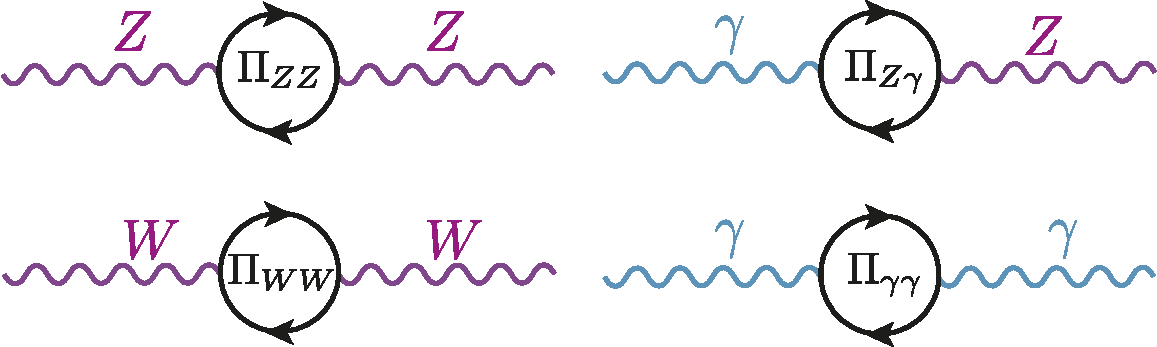
\includegraphics[width=0.75\linewidth]{./figures/oblique_corrections}
	\caption{The oblique corrections, are radiative correction with electroweak gauge bosons propagators. Namely, the vacuum polarisations of the $Z$, $W^\pm$ and $\gamma$ bosons. }  \label{fig:oblique}
\end{figure}
%%%%
%%%%
The one-loop correction to the~$\rho$ parameter is given in terms of the~$\Pi_{VV}$  by
\begin{equation}
	\Delta \rho = \frac{\Pi_{WW}(0)}{m_W^2}- \frac{\Pi_{ZZ}(0)}{m_Z^2}.
\end{equation}
The dominant contributions are given by~\cite{EINHORN1981146}
\begin{align}
	\Delta \rho & = \frac{3 G_F}{8\sqrt{2}\pi^2}\,\left((m_t^2-m_b^2)-\frac{2m_t^2m_b^2}{m_t^2-m_b^2}\ln \frac{m_t^2}{m_b^2} \right)+\dots \ .
	\label{eq:deltarho}
\end{align}
Since $m_b\ll m_t$, the correction is non-vanishing, and~\eqref{eq:deltarho} shows clearly how the radiative corrections are proportional to the spurions of the custodial symmetry. However, this radiative correction is absorbed into the SM definition of $\rho$, i.e. the $\MSbar$ definition of the $\rho$-parameter~$\rho^{\MSbar}$.
\par One can study NP effects violating the custodial symmetry by looking at deviations from $\rho=1$ coming from the NP degrees of freedom. Given the experimentally measured value of~$\rho$~\eqref{eq:rhoexp}, many NP models violating this symmetry can already be excluded. Nevertheless, $\rho$ alone does not capture the full story of~EWPO. For instance, adding a new quark doublet would not necessarily violate the custodial symmetry though it still can be excluded by EWPO. It is hence useful to introduce new parameters known as \textbf{the oblique parameters}~\cite{PhysRevLett.65.2963,PhysRevLett.65.964,PhysRevLett.66.395.2,Peskin91estimationof,peskin1995introduction}~\footnote{The are also called the Peskin–Takeuchi parameters, however, W. Marciano and J. Rosner also D. Kennedy and P. Langacker published the same parametrisation proposals almost simultaneously. Therefore, I preferred not to use this eponym instead of calling them the oblique parameters, as they stem from the oblique corrections.}
\begin{tcolorbox}[title=The oblique parameters,
	title filled=false,
	colback=Mahogany!5!white,
	colframe=Mahogany]
	\begin{align}
		S &:=\frac{4 c_W^2 s_W^2}{\alpha} \left[ \frac{\Pi_{ZZ}^{\NP} (m_Z^2)- \Pi_{ZZ}^{\NP} (0)}{m_Z^2}  - \frac{c_W^2-s_W^2}{c_Ws_W}\,\frac{\Pi_{Z\gamma}^\NP(m_Z^2)}{m_Z^2}-\frac{\Pi_{\gamma\gamma}^\NP(m_Z^2)}{m_Z^2}\right],  \nonumber \\
		T &:=\frac{\rho^{\MSbar}-1}{\alpha}  = \frac{1}{\alpha} \left[ \frac{\Pi^\NP_{WW}(0)}{m_W^2}- \frac{\Pi^\NP_{ZZ}(0)}{m_Z^2} \right] , \\
		U&:= \frac{4 s_W^2}{\alpha} \left[ \frac{\Pi_{WW}^{\NP} (m_W^2)- \Pi_{WW}^{\NP} (0)}{m_W^2}   - \frac{c_W}{s_W}\,\frac{\Pi_{Z\gamma}^\NP(m_Z^2)}{m_Z^2}-\frac{\Pi_{\gamma\gamma}^\NP(m_Z^2)}{m_Z^2}\right] -S .\nonumber 
	\end{align}
\end{tcolorbox}
The NP contributions to the EW vacuum polarisations $\Pi_{VV}^{\NP}(p^2)$) could either come from loop or tree-level effects. Typically both $T$ and $U$ are related to custodial symmetry violation. However, $U$ has an extra suppression factor of $m_\NP^2/m_Z^2$ compared to $T$ and $S$. The most recent fit result for these parameters is~\cite{Zyla:2020zbs}
\begin{align}
	S &=-0.01\pm0.10,  \nonumber \\
	T &= 0.03\pm0.13, \\
	U&:= 0.02\pm0.11.\nonumber 
\end{align}
But since $T$ and $S$ tend to give stronger constraint on NP, as they do not suffer from the suppression that $U$ has. One can preform a two-parameter fit of $S$ and $T$ setting $U=0$; the most recent fit is shown in~\autoref{fig:stubound}, with the best fit values~\cite{Zyla:2020zbs}, \\
\begin{align}
	S &=0.00\pm0.07,  \nonumber \\
	T &= 0.05\pm0.06.
\end{align}
%%%%
\begin{figure}[t]
	\centering
	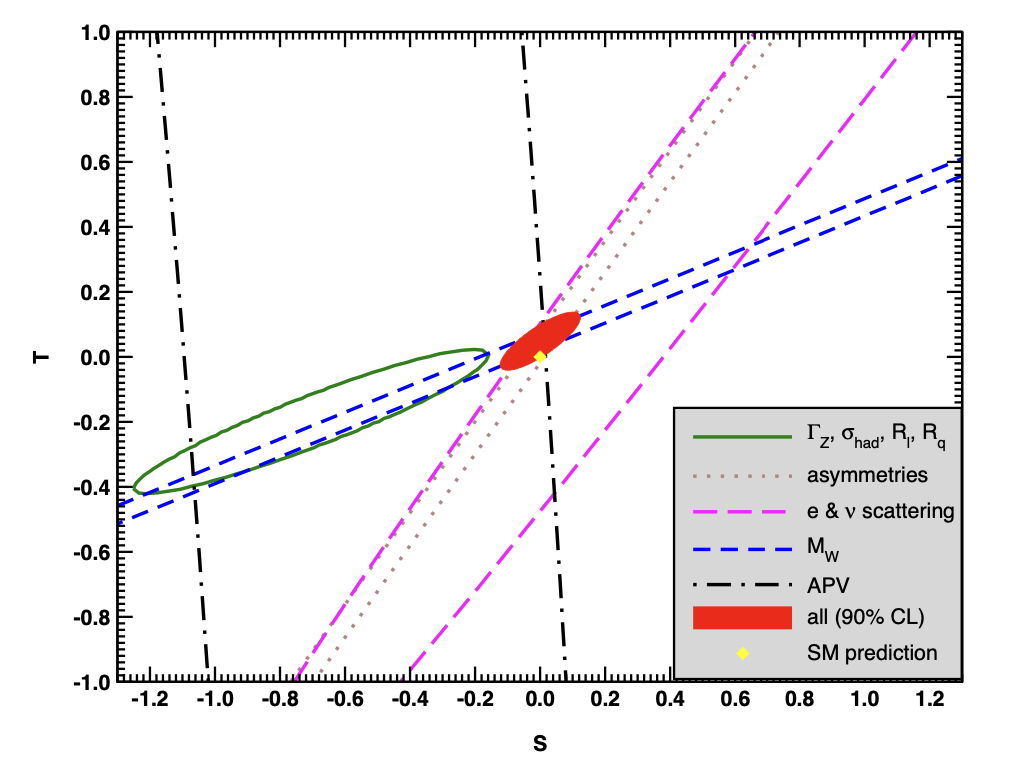
\includegraphics[width=0.65\linewidth]{./figures/stu-pdg}
	\caption{ Fit results from various EWPO's for $T$ and $S$ setting $U=$. The contours show $1\,\sigma$ contours~(39.35\% for closed contours and 68\% for the rest). This plot is obtained from the PDG~\cite{Zyla:2020zbs}.  }  \label{fig:stubound}
\end{figure}
%%%%
%%%%
The oblique parameters are important in constraining effective operators in the Higgs sector, namely
\begin{align}
	\mathcal{O}_S &= \phi^\dagger \sigma_i \phi W^i_{\mu \nu} B^{\mu \nu}, \nonumber \\
	\mathcal{O}_T &= |\phi^\dagger D_\mu \phi|^2.
\end{align}
For example, $\mathcal{O}_S$ appears in Technicolour models causing large deviations of $S$~\cite{GOLDEN19913,HOLDOM199088,ALTARELLI19923,PhysRevLett.65.964}. Moreover,  constraints on the $T$ parameter are important for top mass generation as well as modifications to~$Z  b \bar{b}$ coupling in such models~\cite{PhysRevLett.69.575,Simmons:1995df}. We will revisit these operators when we discuss the Higgs and effective field theories in~\autoref{chap:HiggsEFT}.
\section{Theoretical constraints on the Higgs \label{sec:theoreticalconst}}
\subsection{Electroweak precision data fits }
Even prior to the Higgs boson discovery at LHC,  many theoretical aspects of the Higgs sector provided relatively strong bounds on the Higgs properties, particularly its mass. For instance, using the EWPO measurements at LEP provided input for a fit based on radiative effects coming from the Higgs boson to such observables ~\cite{ALEPH:2005ab} as in diagram (a) of ~\autoref{fig:ewdiagrams}, the bounds improved with the improvements of EWPO measurements, these bounds were known as the ``blue band'' plots seen with their progression in~\autoref{fig:buleband}.
\begin{figure}[t!]
	\begin{center}
		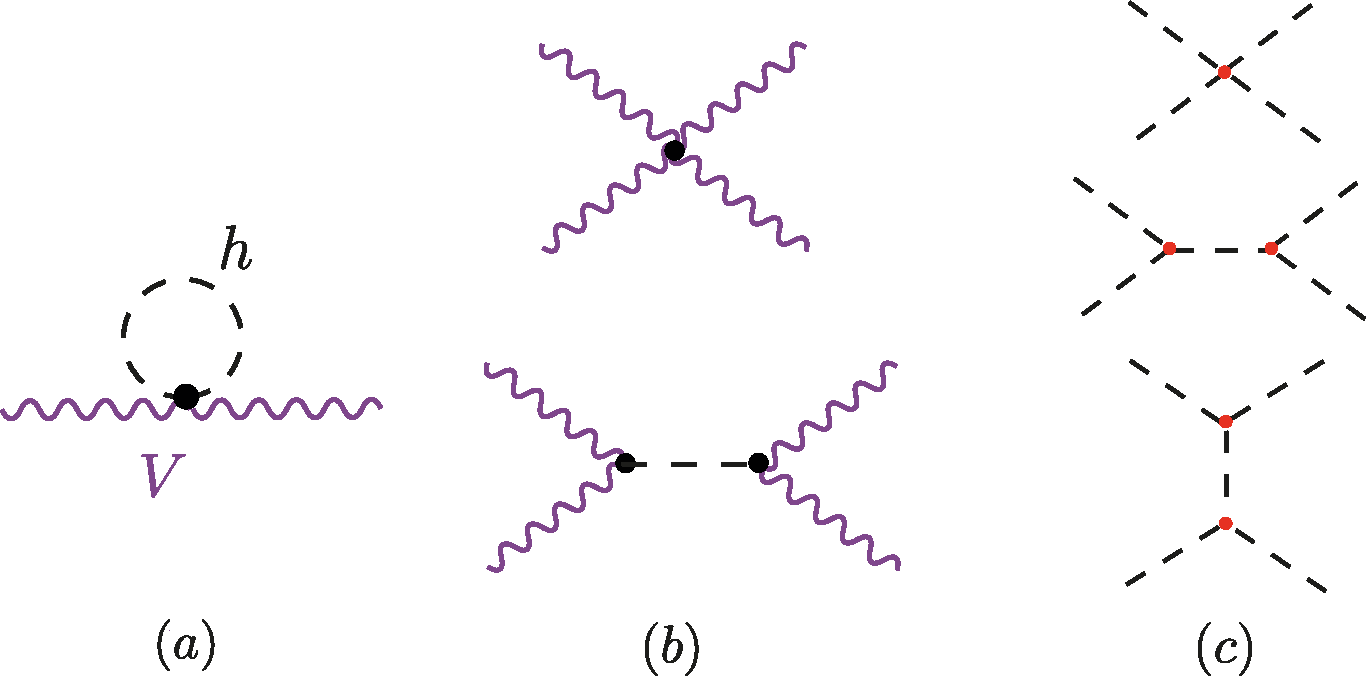
\includegraphics[width=.7 \linewidth]{figures/theoretical_const}
		\caption{Diagrams contributing to theoretical bounds on the Higgs, $(a) $ shows an example of radiative corrections to EWPO from the Higgs boson. The diagrams in $(b)$ show an elastic scattering of EW vector bosons leading to a bound on the Higgs mass from perturbative unitarity, similarly in $(c)$ diagrams for $hh \to hh$ scattering leading to constraints on Higgs self-coupling.}
		\label{fig:ewdiagrams}
	\end{center}
\end{figure}
\begin{figure}[b!]
	\begin{center}
		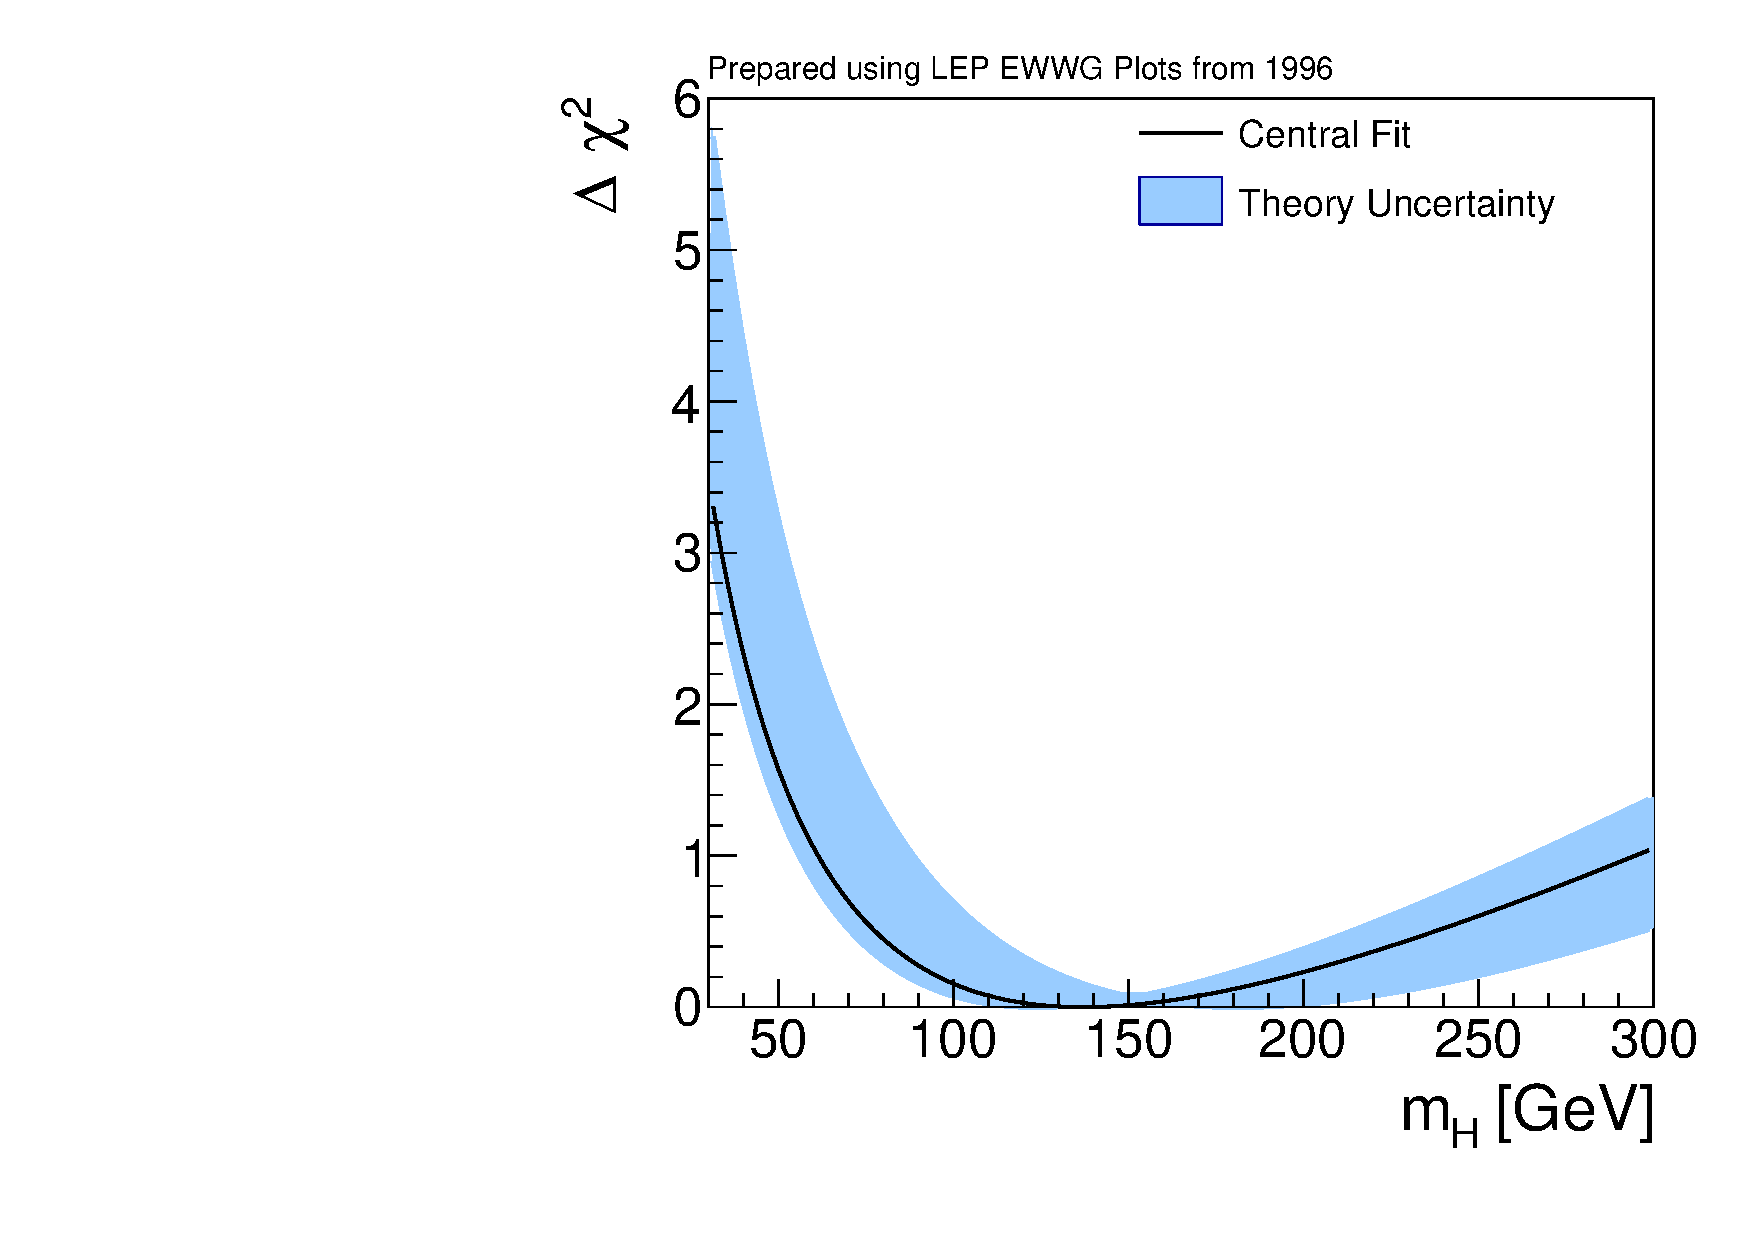
\includegraphics[width=.275 \linewidth]{figures/blueband/BlueBand_1996}
		\hspace{-0.75 cm}
		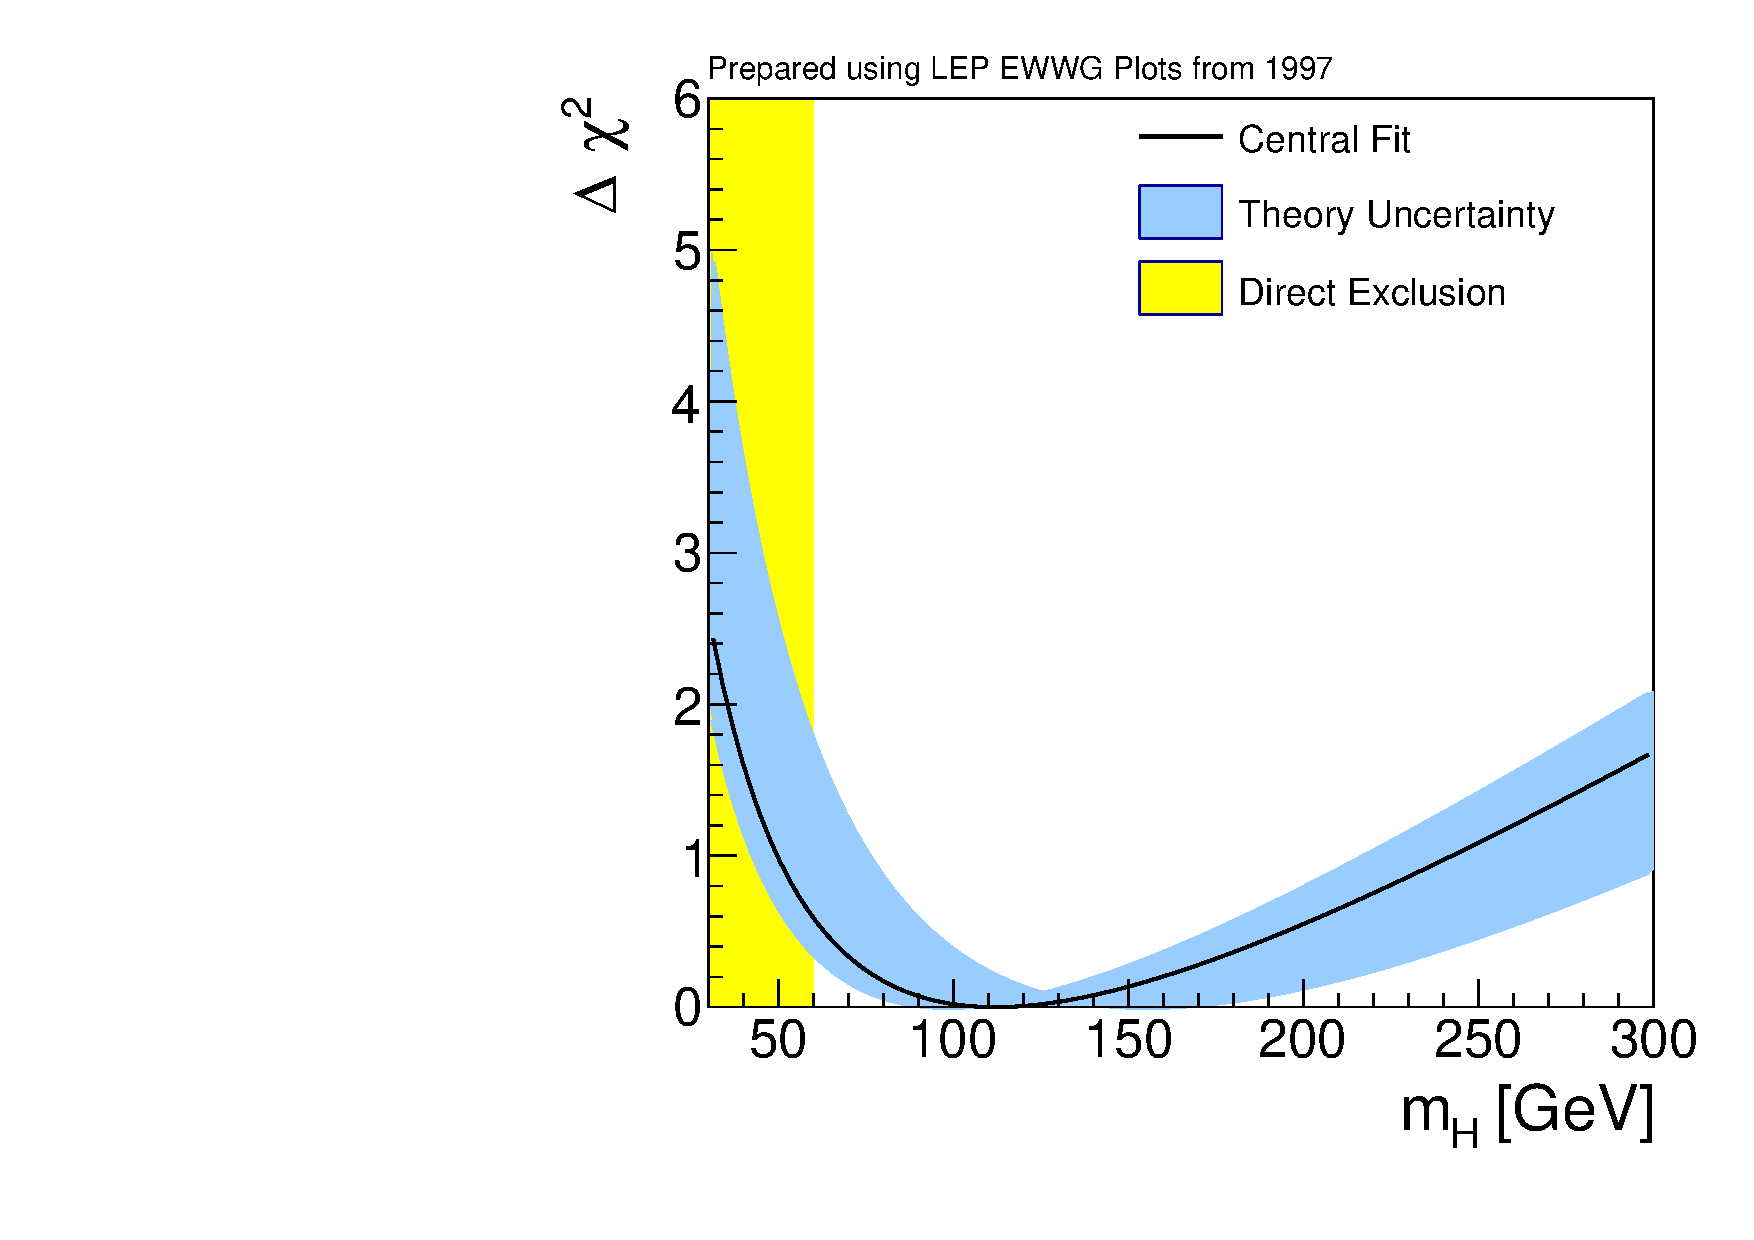
\includegraphics[width=.275 \linewidth]{figures/blueband/BlueBand_1997}
		\hspace{-0.75 cm}
		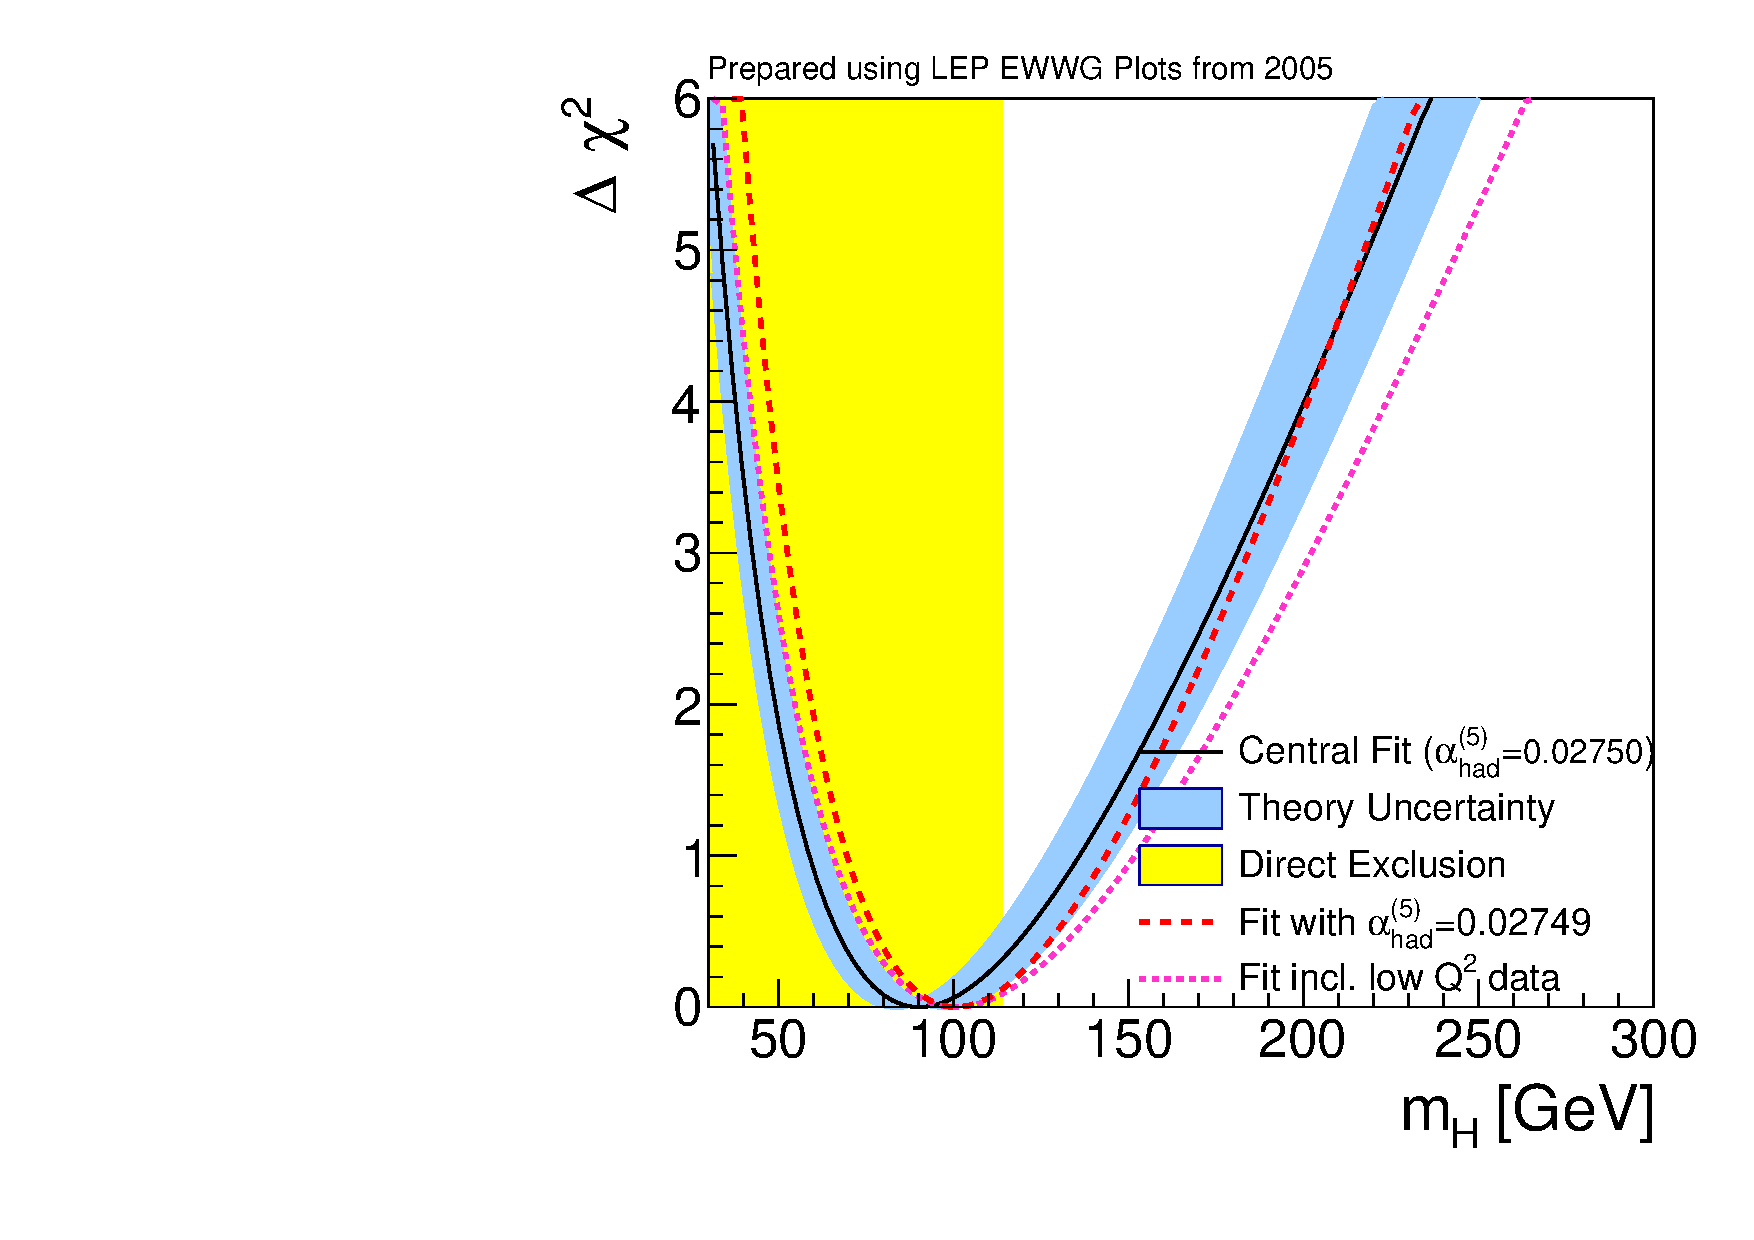
\includegraphics[width=.275 \linewidth]{figures/blueband/BlueBand_2005}
		\hspace{-0.75 cm}
		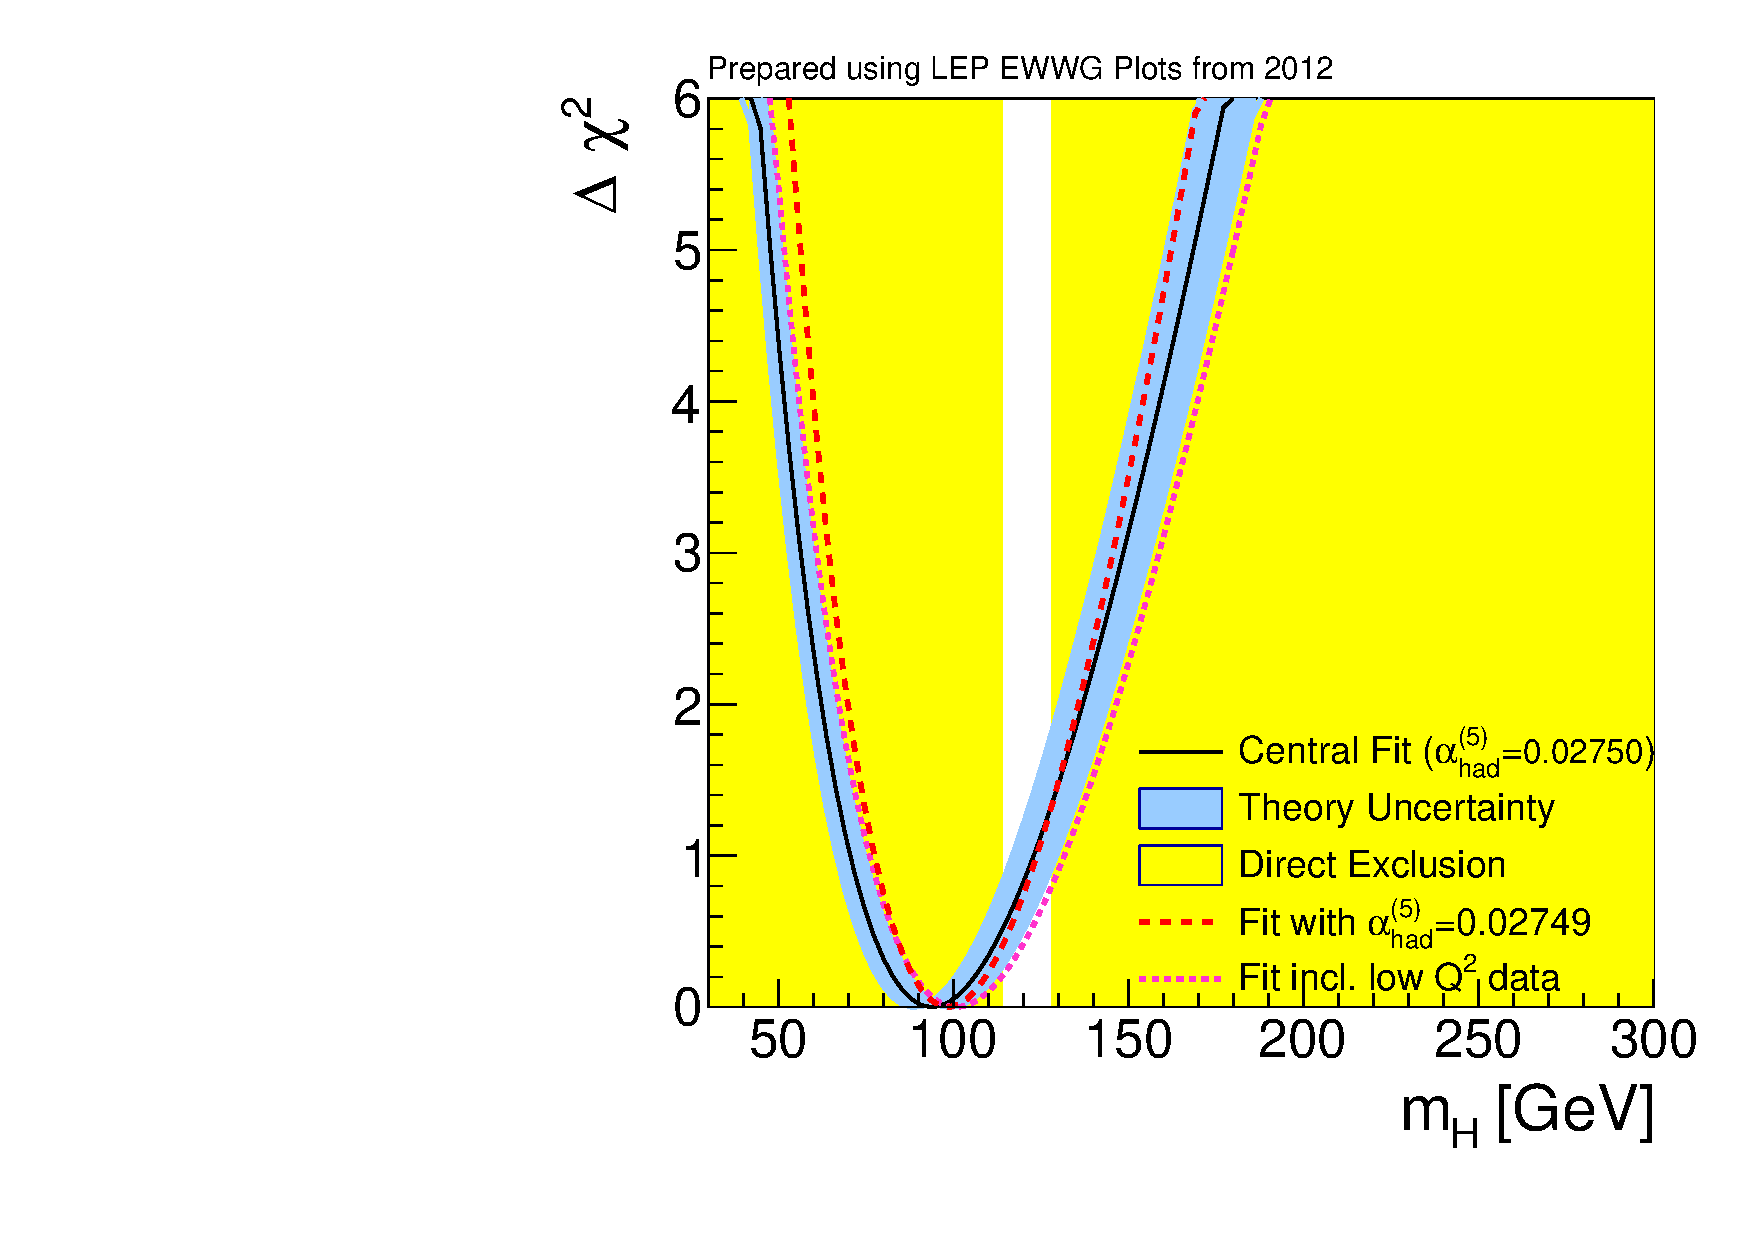
\includegraphics[width=.275 \linewidth]{figures/blueband/BlueBand_2012}
		\caption{Progression of the ``blue band'' plots with LEP data from 1996 up to 2012 prior to the announcement of the Higgs boson discovery. There plots were taken from~\cite{Erler:2019hds}, based data from LEP~\cite{ALEPH:2005ab}. \label{fig:buleband} }
	\end{center}
\end{figure}
\subsection{Partial-wave unitarity \label{pwusection}}
Another bound on Higgs mass emerged from studying the longitudinally polarised elastic scattering amplitudes of the EW vector bosons ~$V_L V_L \to V_L V_L$ at high energies~$ E \gg m_W$, where the Goldstone equivalence theorem holds ~\cite{PhysRevD.42.853}, see diagrams (b) in~\autoref{fig:ewdiagrams}. 
This bound comes from applying the partial wave perturbative unitarity on the EW boson scattering amplitude. I will derive here this bound starting from the \textbf{Optical theorem}, which is a direct result from the unitarity of the $\mathbf S$ matrix.
\begin{tcolorbox}[title=The optical theorem,
	title filled=false,
	colback=Mahogany!5!white,
	colframe=Mahogany]
	Let $\mathcal M_{aa}$ be a covariant matrix element for an elastic  scattering process  for a particle $a \ a \to a \ a$, then the following relation applies
	\begin{equation}
		\sum_{f}  \int d\Phi_n(p_a,p_i^f)| \mathcal M_{af}|^2 = 2 \mathfrak{I}( \mathcal M_{aa}),
		\label{opt}
	\end{equation}
	where the sum is over all intermediate $n$-particle states $f$ with momenta $p_i^f$ and $d\Phi_n(p_a,p_i^f)$ is the $n$-particle phase space.
\end{tcolorbox}
If we only consider a $2 \to 2$ process with momentum states. $\ket{p_1,p_2} \to \ket{k_1,k_2}$, then the LHS of~\eqref{opt}, after expanding the two-particle phase space, simplifies to 
\begin{align}
	&\int  \frac{d^3k_1}{(2 \pi)^3\,2E_1} \int  \frac{d^3k_2}{(2 \pi)^3\,2E_2} (2 \pi)^4 \delta^4(p_1+p_2-k_1-k_2)\,| \mathcal M (s,t)|^2 ,\nonumber \\
	&= \frac{1}{16 \pi} \int_{-1}^{1} d(\cos \theta) | \mathcal M (s,t)|^2,
\end{align}
with the Mandelstam variables 
\begin{align}
	s = &k_1+k_2, \nn \\
	t =& k_1-p_1, \nn \\
	u=& k_1-p_2, \\
	s+t+&u = 4 m^2 . \nn
\end{align}
Using the relation between the Mandelstam variable $t$, and the scattering angle $\theta$:
\begin{equation}
	t = \frac{1}{2} (s-4 m^2)(\cos \theta-1),
\end{equation}
we could expand the matrix element $\mathcal M (s,t)$ in terms of \emph{partial waves}, isolating $s$ from the scattering angle dependence
\begin{equation}
	\mathcal M (s,t) = 16 \pi \sum_j (2j+1)a_j P_j(\cos \theta).
\end{equation}
For each $a_j $ is the $j$th partial wave amplitude, and  $P_j(\cos \theta)$ is the corresponding  Legendre polynomial:
\begin{equation}
	P_j(z) = \frac{1}{j!}\frac{1}{2^j} {d^j\over dz^j} (z^2-1)^j,
\end{equation}
which satisfies the following conditions
\begin{subequations}
	\begin{align}
		\int_{-1}^{1} dz \,P_j(z) P_k(z) &= \frac{1}{2j+1} \delta_{jk}, \\
		P_j(1) &= 1 \,\,\, \forall j.
	\end{align}
\end{subequations}
Applying the afemomentioned relations , one gets for the LHS of \eqref{opt}  
\begin{align}
	&\int  \frac{d^3k_1}{(2 \pi)^3\,2E_1} \int  \frac{d^3k_2}{(2 \pi)^3\,2E_2} (2 \pi)^4 \delta^4(p_1+p_2-k_1-k_2)\,| \mathcal M (s,t)|^2 ,\nonumber \\
	&= \frac{1}{16 \pi} \int_{-1}^{1} d(\cos \theta) \left[ 16 \pi \sum_j (2j+1) a_j(s) P_j(\cos \theta)\right] \times \nonumber\\ & \qquad \left[ 16 \pi \sum_k (2k+1) a_k^*(s) P_k(\cos \theta)\right], \nonumber \\
	& \; = 32 \pi \sum_j (2j+1)| a_j(s)|^2.
\end{align}
Moreover, for the RHS of \eqref{opt}
\begin{equation}
	2 \mathfrak{I}( \mathcal M_{aa}) = \underbrace{2 \mathfrak{I}( \mathcal M(s,0))}_{\color{Mahogany}\text{$t$ is integrated out.}} = 32 \pi  \sum_j (2j+1) \mathfrak{I} (a_j(s)). 
\end{equation}
 The partial-wave amplitudes $a_j(s)$ are  hierarchal, otherwise large cancellations are needed. Thus,  we can compare the partial wave amplitudes term-by-term 
\begin{equation}
	| a_j(s)|^2 \leq \mathfrak{I} (a_j(s)) \;\;\; \Rightarrow \mathfrak{R} (a_j(s))^2+ \mathfrak{I} (a_j(s))^2 \leq \mathfrak{I} (a_j(s)).
\end{equation}
Rearranging terms, we have
\begin{equation}
	\mathfrak{R} (a_j(s)) +\left( \mathfrak{I} (a_j(s))- \frac{1}{2} \right)^2 \leq \frac{1}{4}.
\end{equation}
The partial wave amplitude must  remain within the unitarity circle for the perturbation theory to be valid, i.e.
\begin{equation}
	\mathfrak{R} (a_j(s)) \leq \frac{1}{2}.
	\label{pwu}
\end{equation}
This is known as the perturbative partial wave unitarity constraint.  \\
When~\eqref{pwu} is applied for  $V_L V_L \to V_L V_L$ in the Goldstone boson equivalence theorem regime, in particular for $V=W$ boson, we get for the $S$-wave ($j=0$) partial amplitude
\begin{equation}
	a_0 \sim \frac{m_h^2}{16 \pi  v^2} \left( 2+\mathcal{O} \left(m_h^2/s \right) \right) .
\end{equation}
Looking at the asymptotic behaviour as $ s \to \infty$, the following upper bound on the Higgs mass is obtained
\begin{equation}
	\frac{m_h^2}{8 \pi v^2} < {1\over 2}  \Leftrightarrow  m_h \leq 870 \,\GeV.
\end{equation}
Indeed this bound is obsolete  after the direct Higgs mass detection. However, it is very important to demonstrate the power of this technique in constraining the Higgs boson's parameters. This method can be applied to any elastic scattering with the Higgs  being  the mediator, e.g.  $ZZ\to ZZ$ and  $WW \to ff$. Such processes can be used to constrain their corresponding couplings, i.e. $ g_{ZZh}, g_{f\bar f h}$ and so on. An important bound can be derived by examining the Higgs elastic scattering~$hh \to hh$ shown in $(c)$ of~\autoref{fig:ewdiagrams}, in order to set bounds on Higgs self-interactions~$g_{hhh}$ and $g_{hhhh}$. This is what exactly has been done in ref.~\cite{DiLuzio:2017tfn}, where the authors have found that the $S$-wave partial amplitude for this process is given by
\beq 
\label{a0hhtohh}
a_0= - \frac{1}{2} \frac{\sqrt{s(s-4 m^2_h)}}{16 \pi s} \left[ g_{hhh}^2\left(\frac{1}{s- m_h^2} 
- 2 \frac{\log\frac{s-3m^2_h}{m^2_h}}{s-4m^2_h} \right) + g_{hhhh} \right] \, ,
\eeq
which leads to unitarity bounds on the trilinear~$g_{hhh}$ and the quartic ~$g_{hhhh}$ couplings of:
\beq
\label{unitaritybounds}
\abs{g_{hhh} / g^{\rm SM}_{hhh}} \lesssim 6.5, 
\qquad \text{and} \qquad
\abs{g_{hhhh} / g^{\rm SM}_{hhhh}} \lesssim 65 \, .
\eeq
A more stringent constraint can be obtained by looking at the one-loop correction to the $hh\to hh$ scattering amplitude within the full kinematic range.
The unitarity bound here is obtained by looking at the one-loop  amplitude at the threshold, and is given by
\beq 
\label{pertboundhhhmax}
\abs{g_{hhh} / g_{hhh}^{\text{SM}}} \lesssim 6 \, .
\eeq
It should be noted that the unitarity bound on the trilinear coupling depends on the ansatz that was used for estimating the size of the NP contributions to the scattering amplitudes.
These bounds are, hitherto, the strongest on these two couplings, even when compared to the ones coming from current experimental searches. 
\subsection{Other bounds}
\par Further theoretical bounds can be obtained by studying quantum effects on the Higgs potential. For example, if we looked at the solution of the renormalisation group equation~(RGE) for the Higgs self-coupling~$\lambda$ with the boundary condition $ \lambda(v)=\lambda_0$ and ignoring other SM particle-contributions:
\begin{equation}
	\lambda (Q^2) = \frac{\lambda_0}{1-\frac{3}{4 \pi^2} \log {Q^2\over v^2}}.
	\label{eq_lambdarunnung}
\end{equation}
We see that the running of $\lambda$ will encounter a pole, known as {Landau pole} when the denominator vanishes. This will happen at the scale
\begin{equation}
	Q_{{\rm c}} = v e^{4 \pi^2/3 \lambda_0} =  v e^{4 \pi^2 v^2/3 m_h^2}.
\end{equation}
This indicates that the theory will break down at scales larger or equal to~$ Q_{{\rm c}} $. Since the ``critical scale'' is a function of the Higgs mass, this allows to set an upper limit on the Higgs mass, assuming the SM will be valid up to a certain scale~$ Q_{{\rm c}} $. This is known as \textbf{quantum triviality } constraint~\cite{Lindner:1985uk}. The reasoning behind such constraint stems from the low energy behaviour of ~\eqref{eq_lambdarunnung} leading to a vanishing interaction. If we want the Higgs Lagrangian to be perturbative for all scales, then $\lambda$ has to be vanishing, and the theory becomes non-interacting or \emph{trivial}. 
\par Another bound coming from the RGE of $\lambda$ is the \textbf{stability bound} that considers the stability of the Higgs potential given the running of $\lambda$;  requiring that the Higgs potential is an operator bounded from below. This bound is obtained by approximating the solution of the RGE at small $\lambda$ 
\begin{equation}
	\lambda(Q^2)\sim \lambda_0 +\frac{1}{16 \pi^2} \left[ - \frac{12m_t^4}{v^4} + \frac{3}{16} \left( 2g_2^4+(g_2^2+g_1^2)^2\right) \right] \log{Q^2\over v^2}.
\end{equation}
For the Higgs potential to be bounded from below, $\lambda(Q^2)$ ought to be positive, i.e. $\lambda(Q^2) > 0$. Since $\lambda_0$ can be expressed in terms of the mass, we get a bound on~$m_h$ from this condition
\begin{equation}
	m_h^2 > \frac{v^2}{8 \pi^2} \left[ - \frac{12m_t^4}{v^4} + \frac{3}{16} \left( 2g_2^4+(g_2^2+g_1^2)^2\right) \right] \log{Q^2\over v^2}.
\end{equation}
Leading to $ m_h \approx 130$\ \GeV,\ assuming that the SM is valid up to the Grand Unified Theory~(GUT) scale of $ \sim 10^{16}$ \ \GeV \. Alternatively, the bound becomes $ m_h \approx 180$ \GeV \ for $Q$ being at the Planck scale ~$ \sim 10^{19}$ \ \GeV . 
\par More sophisticated calculations and discussion for the Higgs potential and vacuum stability has been a subject of great interest in pre- and post-Higgs discovery eras cf.~\cite{Lindner:1985uk,Sher:1988mj,Casas:1996aq,Isidori:2001bm}.  The  state-of-the-art calculation for the vacuum stability at two-loop level has been preformed in ref.~\cite{Degrassi:2012ry}, in which, the authors have also included finite temperature effects to construct a phase diagram in the $m_t-m_h$  and $m_t-\lambda(M_{pl})$ planes as shown in~\autoref{fig:vacuum}.  
It indicates that the measured Higgs mass is likely compatible with a metastable vacuum rather than absolute stability. This shows a finite probability for the Higgs vacuum~(false vacuum) to decay into a lower energy state (true vacuum) via quantum tunnelling.
\begin{figure}[t!]
	\begin{center}
		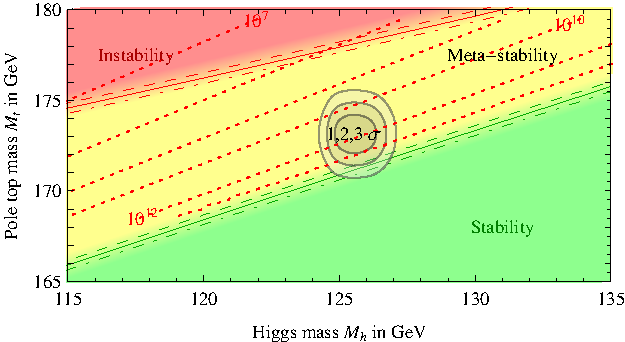
\includegraphics[height=0.32\textwidth]{figures/deadoraliveG2012}
		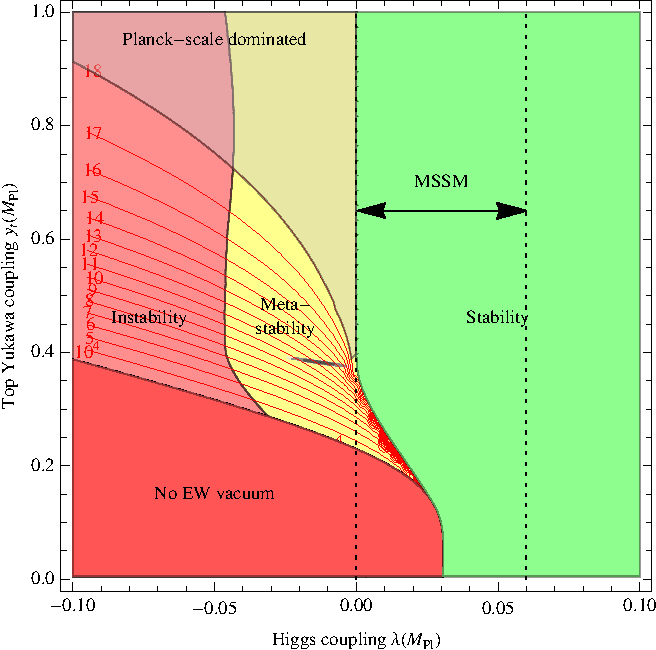
\includegraphics[height=0.32\textwidth]{figures/Ath}
		\caption{Phase diagrams of the Higgs vacuum in the $m_t-m_h$ (left) and  $m_t-\lambda(M_{pl})$ (right) planes showing areas of instability, meta stability and absolute stability. In the  $m_t-\lambda(M_{pl})$ diagram, the allowed range of the Higgs self-coupling $\lambda$ in the Minimal Supersymmetric SM~(MSSM), this plot is taken from ~\cite{Degrassi:2012ry}. }
		\label{fig:vacuum}
	\end{center}
\end{figure}
%%%%%%%%%%%%%%%%%%%%%%%%%%%%%%%%%%%%%%%%%%%%%%%%%%%%%%%%%%%%%%%%%%%%%%%%%%%%%%%%%%%%%%%%%%%%%%%%%%%%%%%%%%%%%%%%%%%%%%
